\section{Komplexe Zahlen}
	\subsection{Definition}
		Die Menge der reellen Zahlen wird auf die Menge der komplexen Zahlen erweitert. $\Rightarrow \mathbb{R} \subset \mathbb{C}$\\
		
		\begin{minipage}[t]{0.5\textwidth}
			\textbf{Komplexe Zahl in Normalform:}\\[3pt]
			\fbox{$z = \underbrace{z_{1}}_{\text{Realteil}} + \underbrace{z_{2}}_{\text{Imaginärteil}} \cdot j$}\\
			$j = \text{imaginäre Einheit}$
		\end{minipage}
		\begin{minipage}[t]{0.5\textwidth}
			\textbf{Komplexe Zahl in Normalform:}\\[3pt]
			\fbox{$z = \underbrace{\left| z \right|}_{Betrag} \cdot \underbrace{[cos(\varphi) + j \cdot sin(\varphi)]}_{Winkel} = r \cdot cjs(\varphi)$}
			$\varphi = \text{Argument } arg(z) \quad\qquad r = \left| z \right| = \text{Betrag}$
		\end{minipage}\\[3pt]
		\textbf{Umrechnung Normal $\rightarrow$ Polar: ($Z_1 \in \mathbb{R}$, $Z_2 \in \mathbb{I}$)}\\
		\begin{tabular}{l}
			\fbox{$|z| = r = \sqrt{z_{1}^2 + z_{2}^2}$}\\[6pt]
			\fbox{$|z| = r = \sqrt{z \cdot \overline{z}}$}\\[6pt]
		\end{tabular}
		\fbox{$\varphi = \left\{
				\begin{array}{ll}
					arctan\left(\dfrac{z_{2}}{z_{1}}\right) & \text{für: } z_{1} \geq 0\\
					arctan\left(\dfrac{z_{2}}{z_{1}}\right) + \pi & \text{für: } z_{1} < 0
				\end{array}
				\right. = \left\{
					\begin{array}{ll}
						\; \; \: arctan\left(\dfrac{z_{1}}{r}\right) & \text{für: } z_{2} \geq 0\\
						-arctan\left(\dfrac{z_{1}}{r}\right) & \text{für: } z_{2} < 0
					\end{array}
				\right.
			$}\\[3pt]
		\scalebox{1}{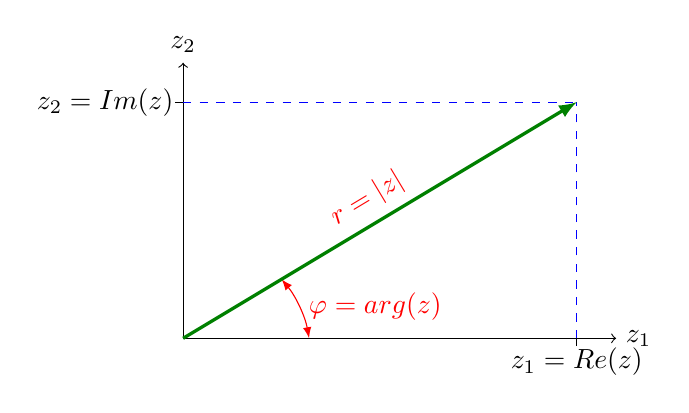
\begin{tikzpicture}
	%\draw[help lines] (0,0) grid (6,4);
	
	\draw [<->] (0, 3.5) -- (0, 0) -- (5.5, 0);
	\node [right] at (5.5, 0) {$z_1$};
	\node [above] at (0, 3.5) {$z_2$};
	
	\draw[latex-latex, red]  (0:1.6) arc(10:40:1.6) node[midway,right]{$\varphi = \operatorname{arg(z)}$};
	
	\draw (5, -0.1) --  (5, 0.1);
	\node [below] at (5, 0) {$z_1 = \operatorname{Re(z)}$};
	
	\draw (-0.1, 3) --  (0.1, 3);
	\node [left] at (0, 3) {$z_2 = \operatorname{Im(z)}$};
	
	\draw [dashed, blue] (0, 3) -- (5, 3);
	\draw [dashed, blue] (5, 0) -- (5, 3);
	
	\draw [-latex, black!50!green, very thick] (0, 0) -- node[sloped, above, red]{$r = \left| z \right|$} (5, 3);
\end{tikzpicture}}\\[3pt]
		\begin{minipage}[t]{0.5\textwidth}
			\textbf{Umrechnung Polar $\rightarrow$ Normal:}\\[3pt]
			\fbox{$z_{1} = r \cdot cos(\varphi)$}
			\fbox{$z_{2} = r \cdot sin(\varphi)$}
		\end{minipage}
		\begin{minipage}[t]{0.5\textwidth}
			\fbox{$\varphi = \left\{
				\begin{array}{ll}
				arctan\left(\dfrac{\mathbb{I}}{\mathbb{R}}\right) & \text{für: } \mathbb{R} \geq 0\\
				arctan\left(\dfrac{\mathbb{I}}{\mathbb{R}}\right) + \pi & \text{für: } \mathbb{R} < 0
				\end{array}
				\right.
				$}\\[3pt]
		\end{minipage}
		\textbf{Sonstige Formeln:}\\[3pt]
		\begin{tabular}{|l|l|}
			\hline
			Moivre'sche Formel & $cjs^n(\varphi) = (cos(\varphi) + j \cdot sin(\varphi))^n = cos(n\varphi) + j \cdot sin(n\varphi) \quad (n \in \mathbb{R})$\\
			\hline
		\end{tabular}\\
		\begin{tabular}{|l|l|l|l|l|}
			\hline
			$\begin{array}{l}
				\mathrm{e}^{\mathrm{j} \pi} = \mathrm{e}^{-\mathrm{j} \pi} = (-1)\\[3pt]
				\mathrm{e}{\mathrm{j} n \pi} = \mathrm{e}{-\mathrm{j} n \pi} = (-1)^n\\[3pt]
			\end{array}$ & $\mathrm{e}^{\mathrm{j} 2 \pi} = \mathrm{e}^{-\mathrm{j} 2 \pi} = 1$ & $\mathrm{e}^{\mathrm{j}\dfrac{\pi}{2}}$ & $\mathrm{j}^{\mathrm{j}} = \mathrm{e}^{-\dfrac{\pi}{2}} + 2 \pi k$ & \\[3pt]
			\hline
			\begin{turn}{90} Potenz \end{turn} \begin{turn}{90} von \end{turn}
			$\left\lbrace \begin{array}{l}
				\mathrm{j} = \sqrt{-1} = j\\[3pt]
				\mathrm{j}^{-1} = -\mathrm{j}\\[3pt]
			\end{array} \right. $ & $(-\mathrm{j})^2 = \mathrm{j}^2 = (-1) \Leftrightarrow \mathrm{j} = \sqrt{-1}$ & $\mathrm{j}^3 = -\mathrm{j}$ & $(-\mathrm{j})^4 = \mathrm{j}^4 = 1$ & $\mathrm{j}^5 = \mathrm{j}^1 \cdots$\\[3pt]
			\hline
			 & $\mathrm{j}^{-2} = -1$ & $\mathrm{j}^{-3} = \mathrm{j}$ & $\mathrm{j}^{-4} = 1$ & $\mathrm{j}^{-5} = \mathrm{j}^{-1}$\\[3pt]		
			\hline
		\end{tabular}\\
	\begin{minipage}[t]{0.5\textwidth}
		\subsection{Konjugierte-komplexe Zahlen}
			\begin{tabular}{c}
				$z = z_{1} + j \cdot z_{2} \xrightarrow[]{konjugieren} \overline{z} = z_{1} - j \cdot z_{2}$\\[3pt]
			\end{tabular}
			\begin{tabular}{|lcl|lcl|}
				\hline
				$\overline{\overline{a}}$ & $=$ & $a$ & $\overline{-a}$ & $=$ & $-\overline{a}$\\
				\hline
				$\overline{a + b}$ & $=$ & $\overline{a} + \overline{b}$ & $\overline{a - b}$ & $=$ & $\overline{a} - \overline{b}$\\
				\hline
				$\overline{a \cdot+ b}$ & $=$ & $\overline{a} \cdot \overline{b}$ & $\overline{a : b}$ & $=$ & $\overline{a} : \overline{b}$\\
				\hline
				$\frac{a + \overline{a}}{2}$ & $=$ & $ Re(a)$ & $\frac{a - \overline{a}}{2j}$ & $=$ & $Im(a)$\\
				\hline
			\end{tabular}
			\begin{tabular}{c}
				\scalebox{1}{\begin{tikzpicture}
	%\draw[help lines] (0,0) grid (6,4);
	\begin{axis}[axis lines=middle, axis equal, grid=both, xlabel = $\operatorname{Re}$, ylabel = $\operatorname{Im}$]
		\addplot[dashed, blue, very thick, mark=*] coordinates{(-2, 2) (2, 2)} node[above, red] at (80, 350) {$\left| -z \right| = -\left| z \right|$};
		\addplot[dashed, blue, very thick, mark=*] coordinates{(-2, -2) (2, -2)} node[above, red] at (375, 355) {$z$};
		\addplot[dashed, blue, very thick, mark=*] coordinates{(-2, 2) (-2, -2)} node[above, red] at (30, 2) {$-z$};
		\addplot[dashed, blue, very thick, mark=*] coordinates{(2, 2) (2, -2)} node[above, red] at (375, 2) {$\left| z \right|$};
	\end{axis}
\end{tikzpicture}}\\[3pt]
			\end{tabular}\\[3pt]
			\fbox{$z \cdot \overline{z} = |z|^2$}\\[3pt]
			\fbox{$(x + \mathrm{j} y) \cdot (x - \mathrm{j} y) = x^2 + y^2$}
	\end{minipage}
	\begin{minipage}[t]{0.5\textwidth}
		\subsection{Addition, Subtraktion}
			\textbf{Normalform:}\\[3pt]
			\fbox{$a + b = (a_{1} + b_{1}) + j \cdot (a_{2} + b_{2})$}\\[3pt]
			\fbox{$a - b = (a_{1} - b_{1}) + j \cdot (a_{2} - b_{2})$}\\[3pt]
		\subsection{Multiplikation, Division}
			\textbf{Normalform:}\\[3pt]
			\fbox{$a \cdot b = (a_{1} \cdot b_{1} - a_{2} \cdot b_{2}) + j \cdot (a_{1} \cdot b_{2} + a_{2} \cdot b_{1})$}\\[3pt]
			\fbox{$a : b = \dfrac{(a_{1} \cdot b_{1} - a_{2} \cdot b_{2})}{b_{1}^2 + b_{2}^2} + j \cdot \dfrac{(a_{1} \cdot b_{2} + a_{2} \cdot b_{1})}{b_{1}^2 + b_{2}^2}$}\\[3pt]
			\scalebox{1}{\begin{tikzpicture}
	%\draw[help lines] (0,0) grid (6,4);
	\begin{axis}[axis lines=middle, axis equal, grid=both, xlabel = $\operatorname{Re}$, ylabel = $\operatorname{Im}$]
		\addplot[->, red, very thick] coordinates{(0, 0) (1, 3)} node[above, red] at (350, 400) {$a-b$};
		\addplot[->, black!50!green, very thick] coordinates{(0, 0) (3, 2)} node[above, black!50!green] at (500, 300) {$a=3+2\mathrm{j}$};
		\addplot[->, red, very thick] coordinates{(0, 0) (5, 1)} node[above, red] at (650, 200) {$a+b$};
		\addplot[->, blue, very thick] coordinates{(0, 0) (2, -1)} node[above, blue] at (500, -70) {$b=2-\mathrm{j}$};
		\addplot[->, dashed, blue, very thick] coordinates{(0, 0) (-2, 1)} node[above, blue] at (25, 200) {$-b$};
	\end{axis}
\end{tikzpicture}}\\[3pt]
	\end{minipage}
	
	\begin{minipage}[t]{0.5\textwidth}
		\subsection{Multiplikation in Polarform}
			\begin{tabular}{l}
				$c = a \cdot b = \left| c \right| \cdot cjs(\varphi_{c})$
			\end{tabular}\\[3pt]
			\begin{tabular}{lcl}
				\fbox{$\left| c \right| = \left| a \right| \cdot \left|b\right| = \left| a \cdot b \right|$} & \fbox{$\varphi_{c} = \varphi_{a} + \varphi_{b}$}
			\end{tabular}\\[3pt]
			\begin{tabular}{l}
				\fbox{$arg(c) = arg(a \cdot b) = arg(a) + arg(b)$}
			\end{tabular}\\[3pt]
			\scalebox{1}{\begin{tikzpicture}
	%\draw[help lines] (0,0) grid (6,4);
	\begin{axis}[axis lines=middle, axis equal, grid=both, xlabel = $\operatorname{Re}$, ylabel = $\operatorname{Im}$]
		\addplot[->, black!50!green, very thick] coordinates{(0, 0) (2, 2)} node[above, black!50!green] at (300, 300) {$a=2+2\mathrm{j}$} node[sloped, rotate = 45, above, black!50!green] at (100, 200) {$|a|$};
		\addplot[->, red, very thick] coordinates{(0, 0) (8, 4)} node[above, red] at (675, 500) {$a \cdot b = 8 + 4\mathrm{j}$} node[sloped, rotate = 25, above, red] at (550, 375) {$|c| = |a \cdot b|$};
		\addplot[->, blue, very thick] coordinates{(0, 0) (3, -1)} node[above, blue] at (400, -70) {$b=3-\mathrm{j}$} node[sloped, rotate = -20, above, blue] at (100, -10) {$|b|$};
		\draw[latex-latex, black!50!green]  ([shift=(60:1cm)]50, 1) arc(0:50:100) node[midway, right, black!50!green]{$\varphi_{1}$};
		\draw[latex-latex, red]  ([shift=(60:1cm)]140, 1) arc(0:50:100) node[midway, right, red] {$\varphi_{2}$};
		\draw[latex-latex, blue]  ([shift=(60:1cm)]100, 1) arc(0:-30:100) node[midway, left, blue] {$\varphi_{3}$};
	\end{axis}
\end{tikzpicture}}\\[3pt]
	\end{minipage}
	\begin{minipage}[t]{0.5\textwidth}
		\subsection{Division in Polarform}
			\begin{tabular}{l}
				$c = \dfrac{a}{b} = \left| c \right| \cdot cjs(\varphi_{c})$
			\end{tabular}\\[3pt]
			\begin{tabular}{lcl}
				\fbox{$\left| c \right| = \dfrac{\left| a \right|}{\left|b\right|} = \left| \dfrac{a}{b} \right|$} & \fbox{$\varphi_{c} = \varphi_{a} - \varphi_{b}$}
			\end{tabular}\\[3pt]
			\begin{tabular}{l}
				\fbox{$arg(c) = arg\left(\dfrac{a}{b}\right) = arg(a) - arg(b)$}
			\end{tabular}\\[3pt]
			\scalebox{1}{\begin{tikzpicture}
	%\draw[help lines] (0,0) grid (6,4);
	\begin{axis}[axis lines=middle, axis equal, grid=both, xlabel = $\operatorname{Re}$, ylabel = $\operatorname{Im}$]
		\addplot[->, red, very thick] coordinates{(0, 0) (1, 2)} node[above, red] at (175, 300) {$c = 1 + 2\mathrm{j}$} node[sloped, rotate = 62.5, above, red] at (65, 225) {$\left|k\right| = \dfrac{a}{b}$};
		\addplot[->, black!50!green, very thick] coordinates{(0, 0) (4, 3)} node[above, black!50!green] at (290, 360) {$a = 4 + 3\mathrm{j}$} node[sloped, rotate = 35, above, black!50!green] at (180, 235) {$|a|$};
		\addplot[->, blue, very thick] coordinates{(0, 0) (2, -1)} node[above, blue] at (260, -10) {$b=2-\mathrm{j}$} node[sloped, rotate = -20, above, blue] at (80, 10) {$|b|$};
		\draw[latex-latex, red]  ([shift=(60:1cm)]20, 40) arc(0:50:1cm) node[midway, right, red]{$\varphi_{1}$};
		\draw[latex-latex, black!50!green]  ([shift=(60:1cm)]100, 40) arc(0:50:100) node[midway, right, black!50!green] {$\varphi_{2}$};
		\draw[latex-latex, blue]  ([shift=(60:1cm)]100, 40) arc(0:-37.5:100) node[midway, right, blue] {$\varphi_{3}$};
	\end{axis}
\end{tikzpicture}}
	\end{minipage}
	
	\subsection{Planare Geometrie mit komplexen Zahlen}
		\begin{minipage}[c]{0.5\textwidth}
			\textbf{Gerade:}\\[3pt]
			\scalebox{0.8}{\begin{tikzpicture}
	%\draw[help lines] (0,0) grid (6,4);
	\begin{axis}[axis lines=middle, axis equal, grid=both, xlabel = $\operatorname{Re}$, ylabel = $\operatorname{Im}$]
		\addplot[red, very thick] coordinates{(-1, -1.5) (7, 2)} node[above, red] at (750, 350) {$g$} node[sloped, rotate = 25, above, red] at (400, 200) {$z_{2} = \dfrac{1}{2}(z_{1} - 2)$};
	\end{axis}
\end{tikzpicture}}
		\end{minipage}
		\begin{minipage}[c]{0.5\textwidth}
			\textbf{Kreis:}\\[3pt]
			\scalebox{0.8}{\begin{tikzpicture}
	%\draw[help lines] (0,0) grid (6,4);
	\begin{axis}[axis lines=middle, axis equal, grid=both, xlabel = $\operatorname{Re}$, ylabel = $\operatorname{Im}$]
		\addplot[->, dashed, red, very thick] coordinates{(3, 1) (2, 3)} node[above, red] at (750, 350) {$g$} node[sloped, rotate = 25, above, red] at (360, 425) {$z_{2} = \dfrac{1}{2}(z_{1} - 2)$};
		\addplot[->, dashed, white] coordinates{(0.5, -2) (0.5, 4)};
		\draw[red] ([shift=(60:1cm)]410, 215) arc(0:360:2.05cm);
	\end{axis}
\end{tikzpicture}}
		\end{minipage}
		
	\subsection{Potenzen und n-te (Einheits-)Wurzeln}
		\subsubsection{Potenzen}
			\begin{minipage}[c]{0.5\textwidth}
				\fbox{$z^n = \underbrace{z \cdot z \cdot \cdots \cdot z}_{\text{n-Faktoren}}, \quad z^0 = 1, \quad z^{-n} = \dfrac{1}{z^n}$}\\[12pt]
				\fbox{$
					\begin{array}{lll}
					z^n & = & \left| z \right|^n \cdot \left[ cos(\varphi) + j \cdot sin(\varphi) \right]^n\\[3pt]
					& = & r^n \cdot \left[ cos(n\varphi) + j \cdot sin(n\varphi) \right]
					\end{array}
				$}
			\end{minipage}
			\begin{minipage}[c]{0.5\textwidth}
				\scalebox{0.8}{\begin{tikzpicture}
	%\draw[help lines] (0,0) grid (6,4);
	\begin{axis}[axis lines=middle, axis equal, grid=both, xlabel = $\operatorname{Re}$, ylabel = $\operatorname{Im}$]
		\addplot[->, black!50!green, very thick] coordinates{(0, 0) (0.5, 0.866)} node[above, black!50!green] at (55, 235) {$a$} node[sloped, rotate = 60, above, black!50!green] at (30, 195) {$|a|$};
		\addplot[->, red, very thick] coordinates{(0, 0) (0.5, -0.866)} node[above, red] at (75, 35) {$b = a^5$} node[sloped, rotate = -60, above, red] at (25, 100) {$\left| b \right| = \left| a^5 \right|$};
		\draw[black!70] ([shift=(60:1cm)]74.5, 103.5) arc(0:360:1.9cm);
		\draw[latex-latex, black!50!green]  ([shift=(60:1cm)]25, 105) arc(0:60:1cm) node[midway, right, black!50!green] {$\varphi_{a}$};
		\draw[latex-latex, red]  ([shift=(60:0.5cm)]12, 128) arc(0:300:0.5cm) node[above, rotate = -60, left, red] at (-10, 90) {$\varphi_{b} = 5 \cdot \varphi_{a}$};
		\addplot[->, dashed, white] coordinates{(0.8, -1.5) (0.8, 1.5)}; % for axis-scaling
	\end{axis}
\end{tikzpicture}}
			\end{minipage}
			
		\subsubsection{n-te Wurzeln}
			\fbox{Di herkömmlichen Wurzelgesetze wie z.B. $\sqrt{a} \cdot \sqrt{b} = \sqrt{a \cdot b}$ gelten nicht mehr!}\\[1pt]
			\begin{minipage}[c]{0.2\textwidth}
				$z = \sqrt[n]{a} = \left| z \right| \cdot cjs(\varphi)$\\[3pt]
				\fbox{$|z|=\sqrt[n]{|a|}$}\\[3pt]
				\fbox{$\varphi_{z}=\frac{\varphi_{a}}{n}$}\\[3pt]
				\fbox{$\arg (z)=\frac{\arg (a)}{n}$}
			\end{minipage}
			\begin{minipage}[c]{0.2\textwidth}
				$\Rightarrow$ \textbf{n-Lösungen!}
			\end{minipage}
			\begin{minipage}[c]{0.3\textwidth}
				$\left\{
					\begin{array}{l}
						z_{1}=\sqrt[n]{r} \cdot \operatorname{cjs}\left(\dfrac{\varphi_{a}}{n}\right) \\[6pt] 
						z_{2}=\sqrt[n]{r} \cdot \operatorname{cjs}\left(\dfrac{\varphi_{a}}{n}+\frac{2 \pi}{n}\right) \\[6pt]
						z_{3}=\sqrt[n]{r} \cdot \operatorname{cjs}\left(\dfrac{\varphi_{a}}{n}+2 \frac{2 \pi}{n}\right) \\[6pt]
						\cdots \\ 
						z_{n}=\sqrt[n]{r} \cdot \operatorname{cjs}\left(\dfrac{\varphi_{a}}{n}+(n-1) \frac{2 \pi}{n}\right)
					\end{array}
				\right.$
			\end{minipage}
			\begin{minipage}[c]{0.2\textwidth}
				\scalebox{0.65}{\begin{tikzpicture}
	%\draw[help lines] (0,0) grid (6,4);
	\begin{axis}[axis lines=middle, axis equal, grid=both, xlabel = $\operatorname{Re}$, ylabel = $\operatorname{Im}$]
		\draw (axis cs: 0, 0) circle [black!10, radius=2];
		\addplot[patch, patch type=triangle, opacity=0.5] coordinates {(-1.73, 1) (1.73, 1) (0, -2)};
		\draw[latex-latex, red]  ([shift=(60:1cm)]330, 175) arc(0:60:1cm) node[midway, rotate=30, right, red] {$\varphi_{z} = \dfrac{\pi}{6}$};
		\addplot[orange, very thick, mark=*] coordinates{(1.73, 1) (1.73, 1)} node[above, red!70] {$z_1 = -\sqrt{3} + \mathrm{j}$};
		\addplot[orange, very thick, mark=*] coordinates{(-1.73, 1) (-1.73, 1)} node[above, red!70] {$z_2 = \sqrt{3} + \mathrm{j}$};
		\addplot[orange, very thick, mark=*] coordinates{(0, -2) (0, -2)} node[above, red!70] {$z_3 = -2\mathrm{j}$};
		\addplot[->, dashed, white] coordinates{(0.8, 1.1) (0.8, 2.5)}; % for axis-scaling
		\addplot[->, dashed, white] coordinates{(0.8, -1) (0.8, -2.5)}; % for axis-scaling
	\end{axis}
\end{tikzpicture}}
			\end{minipage}
		
		\subsubsection{n-te Einheitswurzel}
			\begin{minipage}[t]{0.32\textwidth}
				\begin{tabular}{|l|}
					\hline
					$\displaystyle z = \sqrt[n]{1} = \left| z \right| \cdot \operatorname{cjs}(\varphi_z) = $\\[6pt]
					$\displaystyle |z| \cdot \operatorname{cjs}\left( \dfrac{\varphi_z + k 2 \pi}{n}\right)  = $\\[6pt]
					$\displaystyle \sqrt[n]{|a|} \cdot \operatorname{cjs}\left( \dfrac{\varphi_z + k 2 \pi}{n}\right) $\\[6pt]
					\hline
				\end{tabular}\\[3pt]
				$\Rightarrow$ \textbf{n-Lösungen!}\\[3pt]
				\fbox{$z_n = e_{k}^{(n)} = 1 \cdot \operatorname{cjs\left((k - 1) \cdot \dfrac{2\pi}{n}\right)}$}\\[3pt]
				mit $k = 1, 2, \cdots, n$
			\end{minipage}
			\begin{minipage}[t]{0.12\textwidth}
				\textbf{Es gilt:}\\[3pt]
				$e_{1}^{(n)}=1$\\
				$e_{2}^{(n)}=e_{n}^{(n)}$\\
				$e_{3}^{(n)}=e_{n-1}^{(n)}$\\
				$\cdots$
			\end{minipage}
			\begin{minipage}[c]{0.28\textwidth}
				\scalebox{0.65}{\begin{tikzpicture}
	%\draw[help lines] (0,0) grid (6,4);
	\begin{axis}[axis lines=middle, axis equal, grid=both, xlabel = $\operatorname{Re}$, ylabel = $\operatorname{Im}$]
		\draw (axis cs: 0, 0) circle [black!10, radius=1];
		\addplot[patch, opacity=0.5, table/row sep=\\, patch table={%
			0 1 2\\
			1 2 3\\
			4 3 5\\
		}]
		table[row sep=\\,point meta=\thisrow{c}] {
			x		y		c	\\
			1		0 		1	\\% 0
			0		0		1	\\% 2
			0.31	0.95	0.5	\\% 1
			-0.81	0.59	1	\\% 3
			0		0		0.5	\\% 2
			-0.81	0		1	\\% 4
		};
		\addplot[patch, opacity=0.5, table/row sep=\\, patch table={%
			0 1 2\\
			1 2 3\\
			4 3 5\\
		}]
		table[row sep=\\,point meta=\thisrow{c}] {
			x		y		c	\\
			1		0 		1	\\% 0
			0		0		1	\\% 2
			0.31	-0.95	0.5	\\% 1
			-0.81	-0.59	1	\\% 3
			0		0		0.5	\\% 2
			-0.81	0		1	\\% 4
		};
		\draw[latex-latex, red]  ([shift=(60:1cm)]90, 84) arc(0:55:1cm) node[midway, rotate=30, right, red] {$\varphi = \dfrac{2\pi}{5}$};
		\addplot[orange, very thick, mark=*] coordinates{(1, 0) (1, 0)} node[above, red!70] {$e_1^{(5)}$};
		\addplot[orange, very thick, mark=*] coordinates{(0.31, 0.95) (0.31, 0.95)} node[above, red!70, right] {$e_2^{(5)}$};
		\addplot[orange, very thick, mark=*] coordinates{(-0.81, 0.59) (-0.81, 0.59)} node[above, red!70] {$e_3^{(5)}$};
		\addplot[orange, very thick, mark=*] coordinates{(-0.81, -0.59) (-0.81, -0.59)} node[above, red!70] {$e_4^{(5)}$};
		\addplot[orange, very thick, mark=*] coordinates{(0.31, -0.95) (0.31, -0.951)} node[above, red!70, right] {$e_5^{(5)}$};
		\addplot[->, dashed, white] coordinates{(0.8, 1.1) (0.8, 1.2)}; % for axis-scaling
		\addplot[->, dashed, white] coordinates{(0.8, -1) (0.8, -1.2)}; % for axis-scaling
	\end{axis}
\end{tikzpicture}}
			\end{minipage}
			\begin{minipage}[c]{0.28\textwidth}
				\scalebox{0.65}{\begin{tikzpicture}
	%\draw[help lines] (0,0) grid (6,4);
	\begin{axis}[axis lines=middle, axis equal, grid=both, xlabel = $\operatorname{Re}$, ylabel = $\operatorname{Im}$]
		\draw (axis cs: 0, 0) circle [black!10, radius=1];
		% this uses per-patch color data:
		\addplot[patch, opacity=0.5, table/row sep=\\, patch table={%
			0 1 2\\
			1 2 3\\
			4 3 5\\
		}]
		table[row sep=\\,point meta=\thisrow{c}] {
			x		y		c	\\
			-1		0		0	\\% 0
			-0.5	0.866	1	\\% 1
			0		0 		1	\\% 2
			0.5		0.866 	0	\\% 3
			0		0 		1	\\% 4
			1		0 		1	\\% 5
		};
		\addplot[patch, opacity=0.5, table/row sep=\\, patch table={%
			0 1 2\\
			1 2 3\\
			4 3 5\\
		}]
		table[row sep=\\,point meta=\thisrow{c}] {
			x		y		c	\\
			-1		0		0	\\% 0
			-0.5 	-0.866	1	\\% 1
			0		0 		1	\\% 2
			0.5		-0.866	0	\\% 3
			0		0		1	\\% 4
			1 		0		1	\\% 5
		};
		\draw[latex-latex, red]  ([shift=(60:1cm)]110, 84) arc(0:45:1cm) node[midway, rotate=30, right, red] {$\varphi = \dfrac{2\pi}{6}$};
		\addplot[orange, very thick, mark=*] coordinates{(1, 0) (1, 0)} node[above, red!70] {$e_1^{(6)}$};
		\addplot[orange, very thick, mark=*] coordinates{(0.5, 0.866) (0.5, 0.866)} node[above, red!70] {$e_2^{(6)}$};
		\addplot[orange, very thick, mark=*] coordinates{(-0.5, 0.866) (-0.5, 0.866)} node[above, red!70] {$e_3^{(6)}$};
		\addplot[orange, very thick, mark=*] coordinates{(-1, 0) (-1, 0)} node[above, red!70] {$e_4^{(6)}$};
		\addplot[orange, very thick, mark=*] coordinates{(-0.5, -0.866) (-0.5, -0.866)} node[above, red!70] {$e_5^{(6)}$};
		\addplot[orange, very thick, mark=*] coordinates{(0.5, -0.866) (0.5, -0.866)} node[above, red!70] {$e_6^{(6)}$};
		\addplot[->, dashed, white] coordinates{(0.8, 1.1) (0.8, 1.2)}; % for axis-scaling
		\addplot[->, dashed, white] coordinates{(0.8, -1) (0.8, -1.2)}; % for axis-scaling
	\end{axis}
\end{tikzpicture}}
			\end{minipage}
		
		\subsection{Nullstellen von Polynomen}
			\begin{tabular}{|m{13cm}|}
				\hline
				Ein komplexes Polynom $\operatorname{p}\left(z\right)$ vom Grad $n$ hat 	in $\mathbb{C}$ genau $n$ Nullstellen, wenn diese in ihrem Vielfachen gezählt werden.\\
				$\Rightarrow \quad p_{n}(z)=a_{n} z^{n}+a_{n-1} z^{n-1}+\ldots+a_{0}=a_{n} \cdot\left(z-z_{1}\right) \cdot\left(z-z_{2}\right) \cdot\left(z-z_{3}\right) \cdot \ldots \cdot\left(z-z_{n}\right)$\\
				mit: $z_{1}, z_{2}, z_{3}, \dots, z_{n} \in \mathbb{C}$\\
				\hline
			\end{tabular}
			
			\subsubsection{Polynome mit reellen Koeffizienten}
				\begin{tabular}{|m{13cm}|}
					\hline
					\begin{itemize}
						\item komplexe Nullstellen treten immer als konjugiert-komplexe Paare $(z_0; \overline{z_0})$ mit gleichem Vielfache $k$ auf.
						\item Für die zwei Faktoren gilt $\Rightarrow \quad\left(z-z_{0}\right)(z-\overline{z_{0}})=z^{2}-2 \operatorname{Re}\left(z_{0}\right) \cdot z+\left|z_{0}\right|^{2}$
						\item Im reellen zerfällt $\operatorname{p(z)}$ in \textbf{reelle Linear- und Quadratfunktionen}.
						\item Ist das Polynom von \textbf{ungeradem Grad} $\Rightarrow$ hat es \textbf{mindestens eine reelle Nullstelle}.
					\end{itemize}\\[1pt]
					\hline
				\end{tabular}
		
			\subsubsection{Berechnung der Nullstellen}
				\begin{minipage}[t]{0.7\textwidth}
					\begin{tabular}{|l|}
						\hline
						Alle Nullstellen des Polynoms $p_{n}(z)=a_{n} z^{n}+a_{n-1} z^{n-1}+\ldots+a_{0}$\\
						liegen in der Gauss’schen Zahlenebene in einer Kreisscheibe\\
						um den Ursprung mit Radius:\\
						$\displaystyle r=\sum_{k=0}^{n}\left|\frac{a_{k}}{a_{n}}\right|=\left|\frac{a_{0}}{a_{n}}\right|+\left|\frac{a_{1}}{a_{n}}\right|+\ldots+\left|\frac{a_{n}}{a_{n}}\right|$\\[3pt]
						\hline
					\end{tabular}\\[6pt]
				\end{minipage}
				\begin{minipage}[]{0.3\textwidth}
					\scalebox{0.7}{\begin{tikzpicture}
	%\draw[help lines] (0,0) grid (6,4);
	\begin{axis}[axis lines=middle, axis equal, grid=both, xlabel = $\operatorname{Re}$, ylabel = $\operatorname{Im}$]
		\draw[black!70] ([shift=(60:1cm)]180, 75) arc(0:360:2.58cm);
		\addplot[->, blue, very thick] coordinates{(0, 0) (-0.71, 0.71)} node[above, blue] at (55, 235) {$a$} node[sloped, above, blue] at (30, 195) {$r$};
		\addplot[red, very thick, mark=*] coordinates{(0.8, 0) (0.8, 0)} node[above, red] {$z_1$};
		\addplot[red, dashed, very thick, mark=*] coordinates{(-0.2, -0.8) (-0.2, 0.8)} node[above, red] {$z_2$};
		\addplot[red, dashed, very thick, mark=*] coordinates{(-0.2, 0.8) (-0.2, -0.8)} node[above, red] {$z_3 = \overline{z_2}$};
		\addplot[->, dashed, white] coordinates{(0, 0) (1, -1.1)}; % for axis-scaling
		\addplot[->, dashed, white] coordinates{(0, 0) (-1, 1.1)}; % for axis-scaling
	\end{axis}
\end{tikzpicture}}
				\end{minipage}
				\begin{minipage}[t]{0.3\textwidth}
					\textbf{Quadratische Polynome:}\\[3pt]
					$p(z)=a z^{2}+b z+c=0$\\[3pt]
					\fbox{$\displaystyle z_{1,2}=\frac{-b \pm \sqrt{b^{2}-4 a c}}{2 a}$}
				\end{minipage}
				\begin{minipage}[t]{0.5\textwidth}
					\textbf{Polynome mit $a_{n}=1, a_{n-1}=\ldots=a_{1}=0, a_{0}=a$:}\\[3pt]
					$p(z)=z^{n}+a=0$\\[3pt]
					\fbox{$z_{k}=\sqrt[n]{|a|} \cdot \operatorname{cjs}\left(\frac{\varphi_{a}+\pi}{n}+(k-1) \cdot \frac{2 \pi}{n}\right)$}\\[3pt]
					$\operatorname{mit} k=1,2, \ldots, n$
				\end{minipage}
				\begin{minipage}[t]{0.2\textwidth}
					\textbf{pq-Formel:}\\[3pt]
					$x^{2}+p x+q=0$\\[3pt]
					\fbox{$x_{1,2}=-\frac{p}{2} \pm \sqrt{\left(\frac{p}{2}\right)^{2}-q}$}
				\end{minipage}
			
			\subsection{Komplexe Exponential- und Logarithmusfunktionen}
				\subsubsection{$\mathrm{e}$-Funktion}
					\begin{tabular}{cccccc}
						\fbox{$\mathrm{e}^{\mathrm{j} \varphi}=\cos (\varphi)+\mathrm{j} \sin (\varphi)=\operatorname{cjs}(\varphi)$} 
						&
						$\Rightarrow$
						&
						\fbox{$\begin{aligned} \mathrm{e}^{z} &=\mathrm{e}^{z_{1}+\mathrm{j} z_{2}} \\ &=\mathrm{e}^{z_{1}} \cdot \mathrm{e}^{\mathrm{j} z_{2}} \\ &=\mathrm{e}^{z_{1}} \cdot \mathrm{c} \mathrm{j} \mathrm{s}\left(z_{2}\right) \end{aligned}$}
						&
						$\Rightarrow$
						&
						$\begin{array}{l}
							\text{Betrag:}\\
							\text{Argument}:
						\end{array}$
						&
						$\begin{array}{l}
							\left|\mathrm{e}^{z}\right|=\mathrm{e}^{z_{1}}\\
							\arg \left(e^{z}\right)=z_{2}
						\end{array}$
					\end{tabular}\\
					$\Rightarrow$ \textbf{Potenzgesetze gelten weiterhin!}\\[3pt]
					$\mathrm{e}^{a} \cdot \mathrm{e}^{b}=\mathrm{e}^{a+b} \quad\left|\quad \mathrm{e}^{a}: \mathrm{e}^{b}=\mathrm{e}^{a-b} \quad\right| \quad\left(\mathrm{e}^{a}\right)^{k}=\mathrm{e}^{a \cdot k}$
				
				\subsubsection{Logarithmusfunktionen $\operatorname{Ln}$}
					\begin{minipage}[t]{0.4\textwidth}
						$z=\operatorname{Ln}(a)=z_{1}+\mathbf{j} z_{2}$\\[3pt]
						\fbox{$z_{1}=\ln (|a|)$}
						\fbox{$z_{2}=\varphi_{a}=\arg (a)$}\\[3pt]
						\fbox{$\Rightarrow \quad \operatorname{Ln}(a)=\ln (|a|)+j \arg (a)$}\\[3pt]
					\end{minipage}
					\begin{minipage}[t]{0.6\textwidth}
						\textbf{Lösungen von $\operatorname{Ln}$ sind $\infty$-wertig:}\\[3pt]
						\fbox{$\operatorname{Ln}(a)=\ln (|a|)+\mathbf{j}(\arg (a)+2 k \pi)$}
						mit $k \in \mathbb{Z}$\\[3pt]
						\fbox{$a:= z = z_1 + \mathrm{j} z_2 = x + \mathrm{j} y$}\\[3pt]
					\end{minipage}
					$\Rightarrow$ \textbf{Logarithmusgesetze sind problematisch, da es 1-viele Lösungen gibt!}\\[3pt]
					Es können nur noch Kongruenzen aufgestellt werden (stimmen bis auf ganzzahlige Vielfache von $2 \pi \mathbf{j}$\\[3pt]
					$\operatorname{Ln}(a \cdot b) \stackrel{\bmod 2 \pi \mathrm{j}}{\equiv} \operatorname{Ln}(a)+\operatorname{Ln}(b) \quad|\quad \operatorname{Ln}(a: b) \stackrel{\bmod 2 \pi \mathrm{j}}{=} \operatorname{Ln}(a)-\operatorname{Ln}(b) \quad| \quad \operatorname{Ln}\left(a^{k}\right) \stackrel{\bmod 2 \pi \mathrm{j}}{=} k \cdot \operatorname{Ln}(a)$
				
				\subsubsection{Allgemeine Potenzen}
					\begin{tabular}{cccccc}
						\fbox{$a^{b}=\mathrm{e}^{b \cdot \ln (a)}$}
						&
						$\Rightarrow$
						&
						\textbf{ebenfalls $\infty$-wertige Lösungen!}
						&
						$D = b^2 - 4ac$
						&
						$\Rightarrow$
						&
						$\left\{
							\begin{array}{ll}
								D>0: 
								& 
								2 \text { Lösungen }\\ 
								D=0: 
								& 
								1 \text { Lösung }\\ 
								D<0: 
								& 
								\!\! \text { keine Lösung }
							\end{array}
						\right.$\\
					\end{tabular}\\[3pt]
					\fbox{$\displaystyle z = \mathrm{e}^{\operatorname{Ln}(z)} = \mathrm{e}^{\ln(z) + \mathrm{j} \cdot \operatorname{arg}(z)} = \underbrace{\mathrm{e}^{\ln(z)}}_{|z|} \cdot \underbrace{\mathrm{e}^{\mathrm{j} \cdot \operatorname{arg}(z)}}_{\dfrac{z}{|z|}} = |z| \cdot \dfrac{z}{|z|}$}
					
				\subsection{Komplexe Trigonometrische-Funktionen}
					\begin{tabular}{ccccc}
						\textbf{Trigo:} & \fbox{$\displaystyle \sin (\alpha)=\frac{\mathrm{e}^{\mathrm{j} \alpha}-\mathrm{e}^{-\mathrm{j} \alpha}}{2 \mathrm{j}}$} & \fbox{$\displaystyle \cos (\alpha)=\frac{e^{j \alpha}+e^{-j \alpha}}{2}$} & \fbox{$\displaystyle \tan \alpha=\frac{\sin \alpha}{\cos \alpha}=-j \frac{e^{j \alpha}-e^{-j \alpha}}{e^{j \alpha}+e^{-j \alpha}}$} & \\[4.5mm]
						& \fbox{$\displaystyle \sin(\mathrm{j} \alpha) = \mathrm{j} \sinh(\alpha)$}
						& \fbox{$\displaystyle \cos(\mathrm{j} \alpha) = \cosh(\alpha)$} &&\\[6pt]
						\textbf{Hyperbel:} & \fbox{$\displaystyle \sinh (\alpha)=\frac{\mathrm{e}^{\alpha}-\mathrm{e}^{-\alpha}}{2}$} & \fbox{$\displaystyle \cosh (\alpha)=\frac{\mathrm{e}^{\alpha}+\mathrm{e}^{-\alpha}}{2}$} & \fbox{$\displaystyle \tanh (\alpha)=\frac{\sinh (\alpha)}{\cosh (\alpha)} = \dfrac{\mathrm{e}^\alpha - \mathrm{e}^{-\alpha}}{\mathrm{e}^\alpha + \mathrm{e}^{-\alpha}}$}&\\
					\end{tabular}
				
				\subsection{Komplexe Sinus-Schwingung}
					\begin{tabular}{ll|ll}
						\textbf{Reelle Schwingung:} & & \textbf{Komplexe Schwingung} & \\[3pt]
						\fbox{$\displaystyle z(t)=A \cdot \sin (\omega t+\varphi)$} & & \fbox{$\displaystyle  z(t)=\operatorname{Im}\left[A \cdot \mathrm{e}^{\mathrm{j}(\omega t+\varphi)}\right]=\operatorname{Im}\left[A \cdot \mathrm{e}^{\mathrm{j} \varphi} \cdot \mathrm{e}^{\mathrm{j} \omega t}\right]$} & \\[5pt]
						Amplitude: & $\displaystyle A$ & Komplexe Amplitude (zeitunabhängig): & $\displaystyle A \cdot \mathrm{e}^{\mathrm{j} \varphi}$\\[5pt]
						Nullphasenwinkel: & $\displaystyle \varphi$ & Zeitfunktion (zeitabhängig): & $\displaystyle \left|e^{j \omega t}\right|=1$\\[5pt]
						Kreisfrequenz: & $\displaystyle \omega=2 \pi f$ & & \\[5pt]
						Periodendauer: & $\displaystyle T=\dfrac{2 \pi}{\omega}$ & & \\[5pt]
					\end{tabular}
				
				\subsubsection{Überlagerung von zwei Seiten}
					\begin{minipage}[t]{0.4\textwidth}
						$\displaystyle \begin{aligned} 
							z(t) &=z_{1}(t)+z_{2}(t) \\ &=A_{1} \cdot \sin \left(\omega t+\varphi_{1}\right)+A_{2} \cdot \sin \left(\omega t+\varphi_{2}\right) \\ &=\operatorname{Im}\left[A_{1} \cdot \mathrm{e}^{j\left(\omega t+\varphi_{1}\right)}\right]+\operatorname{Im}\left[A_{2} \cdot \mathrm{e}^{\mathrm{j}\left(\omega t+\varphi_{2}\right)}\right] \\ &=\operatorname{Im}\left[A_{1} \cdot \mathrm{e}^{\mathrm{j} \varphi_{1}} \cdot \mathrm{e}^{\mathrm{j} \omega t}+A_{2} \cdot \mathrm{e}^{\mathrm{j} \varphi_{2}} \cdot \mathrm{e}^{\mathrm{j} \omega t}\right] \\ &=\operatorname{Im}\left[\left(A_{1} \cdot \mathrm{e}^{\mathrm{j} \varphi_{1}}+A_{2} \cdot \mathrm{e}^{\mathrm{j} \varphi_{2}}\right) \cdot \mathrm{e}^{\mathrm{j} \omega t}\right] 
						\end{aligned}$
					\end{minipage}
					\begin{minipage}[]{0.6\textwidth}
						\scalebox{0.65}{\begin{tikzpicture}
	\draw[orange, dashed] (1.4, 1.1) -- (12.15, 1.1);
	\draw[orange, dashed] (1.4, 1.1) -- (1.4, 3.1);
	\draw[orange, dashed] (12.15, 1.1) -- (12.15, 3.1);
	\node[orange] at (6.8, 1.4) {$z(t) = A \cdot e^{\mathrm{j} \varphi} \cdot e^{\mathrm{j} \omega t}$};
	\node[orange] at (1.4, 1.1) {\textbullet};
	\node[orange] at (12.15, 1.1) {\textbullet};
	\draw[orange, dashed] (6.1, 3.8) -- (8.2, 3.8);
	\draw[orange, dashed] (6.1, 3.1) -- (6.1, 3.8);
	\draw[orange, dashed] (8.2, 3.1) -- (8.2, 3.8);
	\node[orange] at (7.2, 4.1) {$z(G) = A \cdot e^{\mathrm{j}\varphi}$};
	\node[orange] at (6.1, 3.8) {\textbullet};
	\node[orange] at (8.2, 3.8) {\textbullet};
	\scalebox{1}{\begin{tikzpicture}
	%\draw[help lines] (0,0) grid (6,4);
	\begin{axis}[axis lines=middle, axis equal, grid=both, xlabel = $\operatorname{Re}$, ylabel = $\operatorname{Im}$]
		\draw[black!70] ([shift=(60:1cm)]180, 75) arc(0:360:2.58cm);
		\addplot[->, blue, very thick] coordinates{(0, 0) (-0.71, -0.71)}  node[sloped, above, blue] {$A$};
		\addplot[->, blue, very thick] coordinates{(0, 0) (0.94, 0.25)}  node[sloped, above, blue] {$A$};
		\addplot[->, dashed, white] coordinates{(0, 0) (1, -1.1)}; % for axis-scaling
		\addplot[->, dashed, white] coordinates{(0, 0) (-1, 1.1)}; % for axis-scaling
	\end{axis}
\end{tikzpicture}}
	\scalebox{1}{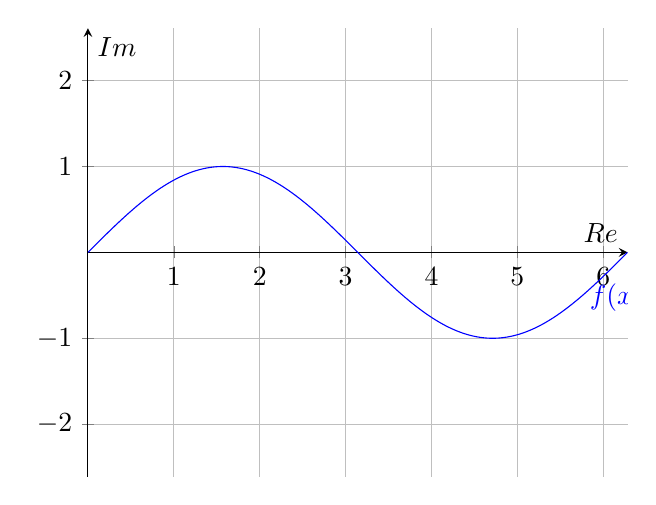
\begin{tikzpicture}
	%\draw[help lines] (0,0) grid (6,4);
	\begin{axis}[axis lines=middle, axis equal, grid=both, xlabel = $\operatorname{Re}$, ylabel = $\operatorname{Im}$]
		\addplot[domain=0:2*pi,samples=200,blue]{sin(deg(x))}node[right,pos=0.9]{$f(x)=\sin x$};
	\end{axis}
\end{tikzpicture}}
\end{tikzpicture}}
					\end{minipage}
					\medskip
					\hrule
					\medskip
					\begin{minipage}[t]{0.5\textwidth}
						\fbox{$\begin{array}{ll}
								\text { reelle Amplitude } & A=\left|A_{1} \cdot \mathrm{e}^{\mathrm{j} \varphi_{1}}+A_{2} \cdot \mathrm{e}^{\mathrm{j} \varphi_{2}}\right| \\ \text { Nullphasenwinkel } & \varphi=\arg \left(A_{1} \cdot \mathrm{e}^{\mathrm{j} \varphi_{1}}+A_{2} \cdot \mathrm{e}^{\mathrm{j} \varphi_{2}}\right)
							\end{array}$}
					\end{minipage}
					\begin{minipage}[]{0.5\textwidth}
						\scalebox{0.65}{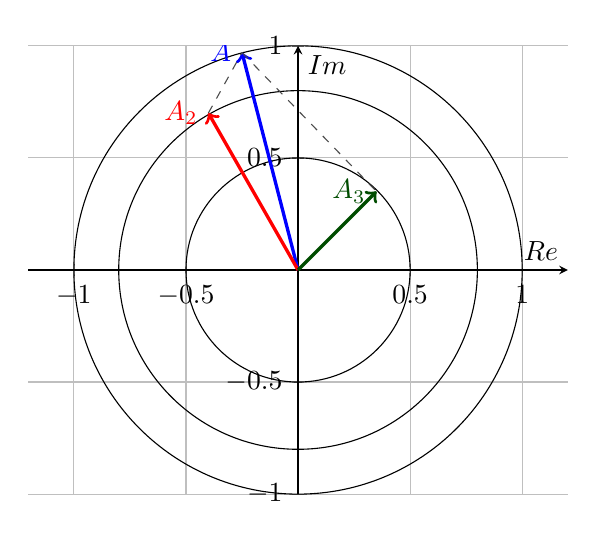
\begin{tikzpicture}
	%\draw[help lines] (0,0) grid (6,4);
	\begin{axis}[axis lines=middle, axis equal, grid=both, xmin=-1, xmax=1, ymin=-1, ymax=1, xlabel = $\operatorname{Re}$, ylabel = $\operatorname{Im}$]
		\draw (axis cs: 0, 0) circle [blue, radius=1];
		\draw (axis cs: 0, 0) circle [red, radius=0.8];
		\draw (axis cs: 0, 0) circle [black!70!green, radius=0.5];
		\addplot[->, blue, very thick] coordinates{(0, 0) (-0.25, 0.97)}  node[sloped, above, blue, left] {$A$};
		\addplot[->, red, very thick] coordinates{(0, 0) (-0.4, 0.7)}  node[sloped, above, red, left] {$A_2$};
		\addplot[->, black!70!green, very thick] coordinates{(0, 0) (0.35, 0.35)}  node[sloped, above, black!70!green, left] {$A_3$};
		\addplot[dashed, black!70] coordinates{(-0.4, 0.7) (-0.25, 0.97)};
		\addplot[dashed, black!70] coordinates{(-0.25, 0.97) (0.35, 0.35)};
	\end{axis}
\end{tikzpicture}}
					\end{minipage}
